\chapter{Proposta de trabalho}

Este capítulo evidencia o que será desenvolvido, ou seja, a proposta inicial do software PGTBL.

Recapitulando, o objetivo do projeto é a automatização do metodologia ativa de aprendizagem baseada em equipe ou TBL, essa metodologia é uma estratégia de ensino colaborativa que se concentra em um ciclo de três passos:

\begin{enumerate}
  \item \textbf{Preparação}: Basicamente o professor irá disponibilizar de artigos e livros para estudo que será a preparação para as avaliações.
  \item \textbf{Avaliação em classe}: A primeira avaliação é individual e a segunda em grupo para testar o conhecimento adquirido na preparação e o trabalho em equipe respectivamente.
  \item \textbf{Pequeno projeto centrado na aplicação}: Aplicar todo o conhecimento adquirido em um contexto real no tópico proposto.
\end{enumerate}

\section{Finalidade}

A finalidade do software é que a aplicação do TBL se torne algo mais fácil, constante e automatizado, tornando o processo mais prazeroso, tanto para o aluno quanto para o professor. A ideia do sistema é ter um design atrativo e será responsável por todo o processo do TBL desde a preparação até as avaliações e fechamento da disciplina.

\section{Descrição dos usuários}

\begin{table}[h!]
  \centering
  \caption{Descrição do usuário professor}
  \label{tab:18}
  \begin{tabular}{@{}ll@{}}
    \toprule
    \multicolumn{2}{l}{\textbf{Professor}}
    \\ \midrule
    \textbf{Descrição:}        & \begin{tabular}[c]{@{}l@{}}Pessoas que busca melhorar o ensino e a forma de avaliação
    das\\ escolas e universidades.\end{tabular}                                                \\
    \textbf{Responsabilidade:} & \begin{tabular}[c]{@{}l@{}}Gerenciamento das disciplinas e alunos usando o sistema.\\ O
    professor também é responsável por criar e gerenciar\\ listas e avaliações.\end{tabular} \\
    \textbf{Critérios de sucesso:} & \begin{tabular}[c]{@{}l@{}}Permite que os alunos possam aprender de uma maneira\\
    mais ativa e colaborativa.\end{tabular}                               \\
    \textbf{Envolvimento:}     & Alto
    \\ \bottomrule
  \end{tabular}
\end{table}

\begin{table}[h!]
  \centering
  \caption{Descrição do usuário monitor}
  \label{tab:19}
  \begin{tabular}{@{}ll@{}}
    \toprule
    \multicolumn{2}{l}{\textbf{Monitores}}
    \\ \midrule
    \textbf{Descrição:}            & \begin{tabular}[c]{@{}l@{}}Alunos ou professores que buscam ajudar na aplicação\\
    do TBL dentro da plataforma.\end{tabular}                                      \\
    \textbf{Responsabilidade:}     & \begin{tabular}[c]{@{}l@{}}Gerenciar questões da lista de exercícios, arquivos da\\
    disciplina e das sessões de TBL, tirar dúvidas, entre\\ outras.\end{tabular} \\
    \textbf{Critérios de sucesso:} & \begin{tabular}[c]{@{}l@{}}Permite que os alunos possam aprender de uma maneira\\
    mais ativa e colaborativa\end{tabular}                                         \\
    \textbf{Envolvimento:}         & Médio
    \\ \bottomrule
  \end{tabular}
\end{table}

\begin{table}[h!]
  \centering
  \caption{Descrição do usuário Aluno}
  \label{tab:20}
  \begin{tabular}{@{}ll@{}}
    \toprule
    \multicolumn{2}{l}{\textbf{Alunos}}
    \\ \midrule
    \textbf{Descrição:}            & \begin{tabular}[c]{@{}l@{}}Pessoas que queiram aprender e se preparar para o
    mercado\\ de trabalho de forma colaborativa e não competitiva\end{tabular} \\
    \textbf{Responsabilidade:}     & Fazer todas as atividades relacionadas ao TBL.
    \\
    \textbf{Critérios de sucesso:} & \begin{tabular}[c]{@{}l@{}}Aprender as disciplinas e se sentir preparado para
    atuar\\ no mercado.\end{tabular}                                          \\
    \textbf{Envolvimento:}         & Alto
    \\ \bottomrule
  \end{tabular}
\end{table}

\section{Principais necessidades dos usuários}

\subsection{Gerenciar aulas}

\begin{itemize}
  \item \textbf{Necessidade}: Gerenciar aulas
  \item \textbf{Prioridade}: Alta
  \item \textbf{Preocupações}: Conseguir gerenciar as aulas através do software PGTBL
  \item \textbf{Solução proposta}: Software que ajude na aplicação da metodologia.
  \item \textbf{Solução atual}: Ensino com pouca participação do aluno e avaliações ineficientes do conhecimento.
\end{itemize}

\subsection{Aprender}

\begin{itemize}
  \item \textbf{Necessidade}: Aprender
  \item \textbf{Prioridade}: Alta
  \item \textbf{Preocupações}: Os alunos devem sair das universidades preparados para o mercado de trabalho
  \item \textbf{Solução proposta}: Software que faça o aluno ser mais ativo nas aulas e aprenda a trabalhar em equipe.
  \item \textbf{Solução atual}: Alunos pouco motivados a se preparar para o mercado de trabalho.
\end{itemize}

\section{Visão geral do produto}

Este sistema tem como objetivo inovar a forma como as escolas/universidades ensinam seus alunos através do TBL, fazendo com que eles tenham uma preparação mais adequada para atuar no mercado, tendo a participação ativa dos alunos e aprimorando seu trabalho em equipe.

\subsection{Recursos do produto (Requisitos funcionais ou Épicos)}

\begin{table}[h!]
  \centering
  \caption{Requisitos Funcionais ou Épicos do produto}
  \label{tab:21}
  \begin{tabular}{@{}ll@{}}
    \toprule
    \textbf{Recurso}                                                           & \textbf{Descrição}
    \\ \midrule
    \begin{tabular}[c]{@{}l@{}}Administrar Disciplinas\\ e alunos\end{tabular} & \begin{tabular}[c]{@{}l@{}}O professor
      pode adicionar, remover, criar e editar disciplinas\\ e turmas e disponibilizar a senha de acesso a elas para os
  alu-\\ nos entrarem, além de poder remover ou adicionar estudantes\\ na turma e gerenciar suas notas.\end{tabular}
  \\ \midrule
  Criar conta                                                                & \begin{tabular}[c]{@{}l@{}}O professor e
    os alunos pode criar sua contas no sistema,\\ apenas passando seus dados pessoais como nome, email,\\ senha, e
  usuário\end{tabular}
  \\ \midrule
  \begin{tabular}[c]{@{}l@{}}Gerenciar dados\\ pessoais\end{tabular}         & \begin{tabular}[c]{@{}l@{}}O usuário
poderá editar sua senha e dados pessoais do\\ usuário conforme necessário.\end{tabular}
\\ \midrule
\begin{tabular}[c]{@{}l@{}}Funcionalidades do\\ TBL\end{tabular}           & \begin{tabular}[c]{@{}l@{}}Funcionalidades
  relacionadas às fases de preparação, garantia\\ de preparo ou RAT, iRAT, gRAT e apelações, Aplicação de\\ conceitos e
  avaliação em pares\end{tabular}                                                                                   \\
  \midrule
  Relatório                                                                  & \begin{tabular}[c]{@{}l@{}}O professor
    terá um dashboard com relatórios do desempenho\\ dos alunos em cada questão da avaliação, tendo um feedback\\ para o
  que ele deve focar mais nas aulas.\end{tabular}
  \\ \midrule
  Rank e Gamificação                                                         & \begin{tabular}[c]{@{}l@{}}Terá também um
    rank de grupos, na qual o primeiro colocado\\ ficará exposto no Hall da Fama que será visto por novos alunos\\ dos
    próximos semestres, não há rank individual porque o obje-\\ tivo não é a competição e sim a
  colaboração.\end{tabular} \\ \bottomrule
  \end{tabular}
\end{table}

\subsection{Restrições}

A proposta do serviço ofertado, envolve a utilização de certos recursos que necessitam de um navegador. De modo que tais recursos implicam em certas limitações do produto, estas limitações seriam:

\begin{itemize}
  \item O usuário deve dispor de um provedor de internet;
  \item O usuário deve dispor de um navegador;
\end{itemize}

\section{Requisitos de qualidade (Não funcionais ou Enables)}

\begin{itemize}
  \item \textbf{Sistema}: O sistema deve seguir a arquitetura MVC definida no documento de Arquitetura e as ferramentas de desenvolvimento será o Python (versão 3.5) e o framework Django (versão 1.11) tendo atualização constante.
  \item \textbf{Suportabilidade}: O sistema poderá ser acessado em computadores pessoais - notebook, desktop – utilizando-se de um serviço de internet. Sendo uma aplicação Web compatível com os principais sistemas operacionais (Linux, Mac, Windows), acessada através do navegador Google Chrome e/ou Firefox de um dispositivo móvel ou fixo.
  \item \textbf{Qualidade}: O sistema deve seguir uma folha de estilo a ponto de o código ser legível e de fácil manutenção, tendo como base boas práticas de programação, o sistema deve ter baixo acoplamento e alta coesão além de ser modularizado focando na flexibilidade e manutenção do mesmo.
  \item \textbf{Usabilidade}: O sistema deve ser responsivo, adaptando-se à plataforma que o usuário estiver utilizando e o design deve ser fácil de usar e aprender e seguir todos as heurísticas de usabilidade.
  \item \textbf{Desempenho}: Por ser um sistema web o software necessita de uma conexão estável com a internet para seu funcionamento. A velocidade da internet tem impacto direto no desempenho da aplicação, sendo necessário uma velocidade suficiente para processar as informações e executar as funcionalidades do sistema.
  \item \textbf{Segurança}: O sistema deve apresentar uma boa percentagem de cobertura de testes, mínimo de 70% e bastante encapsulamento de código, além de um sistema de log eficiente e ter confiabilidade.
  \item \textbf{Confiabilidade}: O sistema deve se comprometer em apresentar informações confiáveis para o usuário do sistema, entretanto dependerá diretamente dos demais usuários, uma vez que o conteúdo apresentado será de autoria destes e deve apresentar um sistema de autenticação, autorização e recuperação seguro e eficiente.
\end{itemize}

\section{Alternativas e Concorrências}

Não foi encontrada nenhum site que automatiza as tarefas do \textit{Team Based Learning}, apenas artigos, livros e sites ensinando como aplicar o TBL dentro das universidades e escolas usando apenas papel e caneta.

\begin{itemize}
  \item \href{https://aprender.unb.br/}{Moodle}: Mesmo que siga a mesma ideia do software proposto o moodle normalmente serve só para disponibilizar informações e arquivos relevantes para os alunos.
  \item \href{https://iesb.blackboard.com/}{Blackboard IESB}: Também segue a mesma ideia, mas não aplica conceitos do Team Based Learning.
\end{itemize}

\section{Ferramentas e Tecnologias}

Abaixo será listado todas as ferramentas e tecnologias utilizadas para a realização do projeto.

\begin{itemize}
  \item \textbf{Draw.io}: Criação de diagramas.
  \item \textbf{Google Drive}: Armazenamento e edição colaborativa dos artefatos e documentos do projeto.
  \item \textbf{Git e Github}: Controle de versão do código para um bom gerenciamento do mesmo.
  \item \textbf{Zenhub}: Permitir o gerenciamento constante das tarefas que serão realizadas durante o projeto.
  \item \textbf{Linux}: Ambiente de desenvolvimento, homologação, produção e teste.
  \item \textbf{Whatsapp e Email}: Permite a comunicação entre os membros da equipe e os stakeholders, além da
    comunicação presencial.
  \item \textbf{Travis CI}: Ferramenta responsável por realizar a integração contínua das funcionalidades realizadas
  \item \textbf{Codacy}: Ferramenta para cobertura de testes e análise estática de código, usado para coletar métricas e
    melhorar a qualidade do código.
  \item \textbf{Docker}: Ferramentas responsáveis por criar um ambientes de desenvolvimento, teste, homologação e produção
  \item \textbf{DockerHub}: Ferramenta para armazenar as imagens de cada ambiente.
  \item \textbf{Python}: Linguagem de programação para a criação do software na versão 3.5.
  \item \textbf{Django}: Framework utilizado para a criação do software na versão 1.11.
  \item \textbf{Makefile}: Usado para facilitar a execução de scripts.
  \item \textbf{mkdocs}: Usado para criar a documentação do software.
\end{itemize}

\section{EAP e ROADMAP}

O projeto tem como base dois principais marcos definidos na tabela \ref{tab:22}, que representam entregas do produto, são eles: \textit{Release 01} e \textit{Release 02}.

\begin{table}[h!]
  \centering
  \caption{Marcos do projeto}
  \label{tab:22}
  \begin{tabular}{@{}lll@{}}
    \toprule
    \textbf{Marco}             & \textbf{Data} & \textbf{Atividade}
    \\ \midrule
    \textbf{Início do projeto} & 03/10/2017    & Começo do projeto
    \\ \midrule
    \textbf{Release 01}        & 01/08/2018    & \begin{tabular}[c]{@{}l@{}}Entrega da primeira versão funcional do
    sistema\\ com algumas funcionalidades implementadas e\\ testadas, além de sua documentação\end{tabular}           \\
    \midrule
    \textbf{Release 02}        & 01/03/2019    & \begin{tabular}[c]{@{}l@{}}Entrega do versão final do projeto com as
    funcio-\\ nalidades restantes do escopo previamente definido\\ com a utilização da abordagem ágil.\end{tabular} \\
    \bottomrule
  \end{tabular}
\end{table}

\subsection{EAP - Estrutura Analítica do Projeto}

A Estrutura Analítica do Projeto ou EAP, foi utilizada como entrada do processo fornecendo os pacotes de trabalho previamente discutidos. Esses pacotes foram então decompostos de maneira a gerar suas respectivas atividades.

\begin{figure}[h!]
	\centering
  \includegraphics[keepaspectratio=true,scale=0.15]{figuras/EAP.eps}
  \caption{EAP do projeto}
	\label{fig:eap}
\end{figure}

\subsection{ROADMAP}

Roadmap definido na figura \ref{fig:roadmap1} e figura \ref{fig:roadmap2} é uma ferramenta muito útil para gestores de produto. Com ele é possível planejar e comunicar a visão de futuro que vc tem para o seu produto. É o cronograma da metodologia ágil.

\begin{figure}[h!]
	\centering
  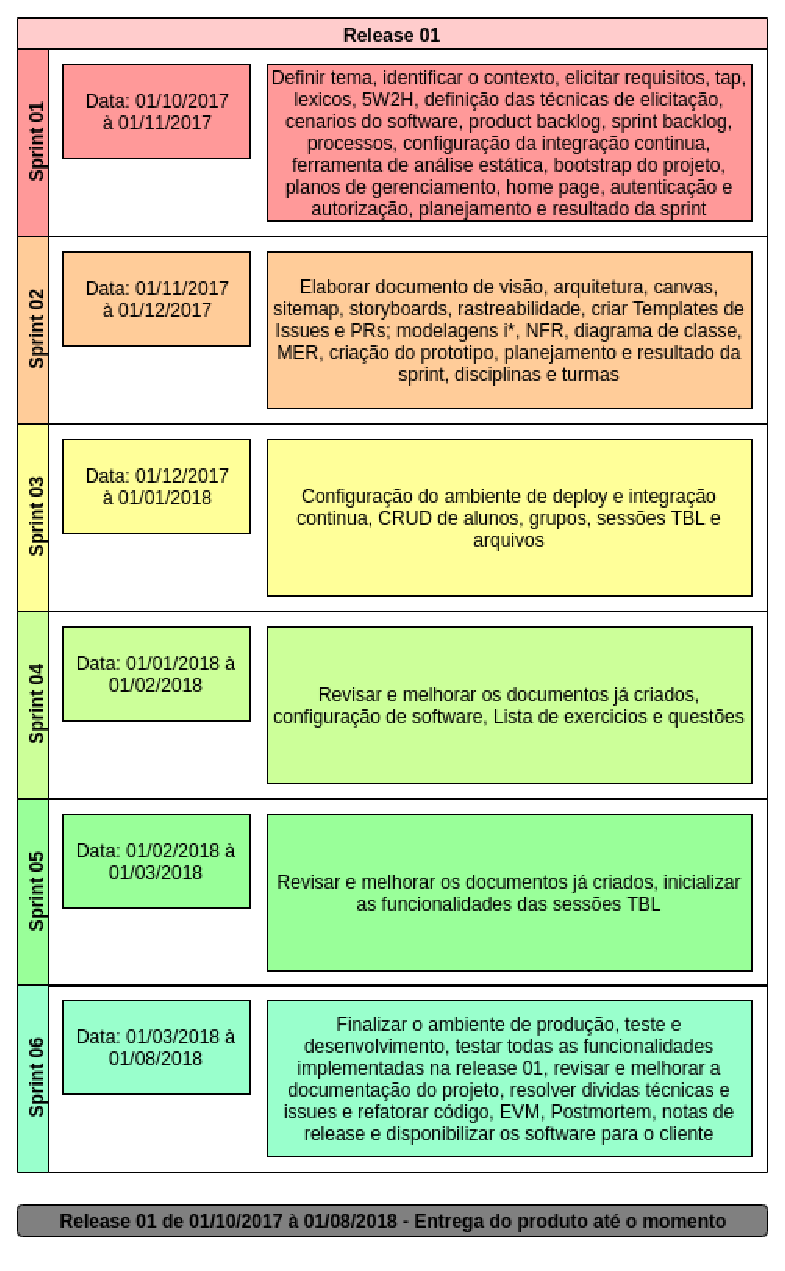
\includegraphics[keepaspectratio=true,scale=0.8]{figuras/roadmap.eps}
  \caption{Roadmap da release 01}
	\label{fig:roadmap1}
\end{figure}

\begin{figure}[h!]
	\centering
  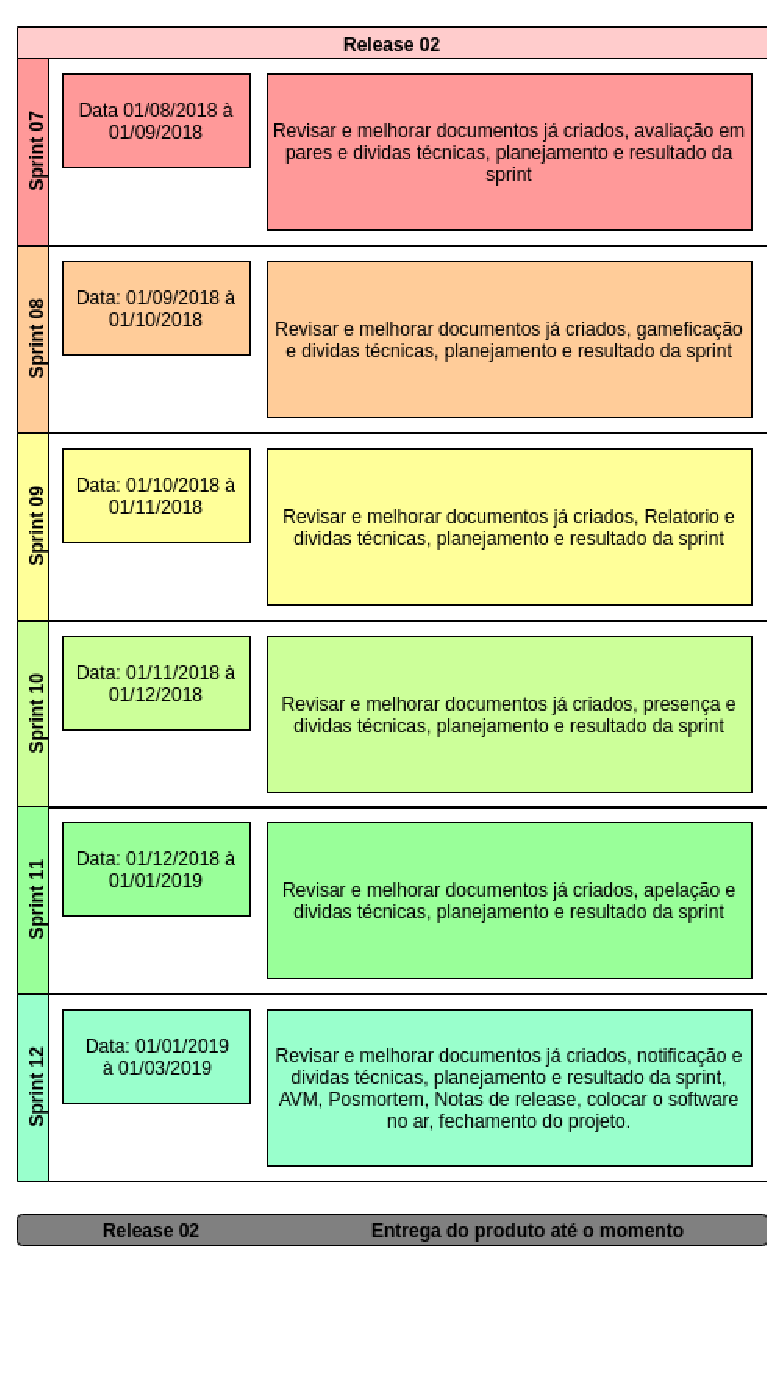
\includegraphics[keepaspectratio=true,scale=0.8]{figuras/roadmap2.eps}
  \caption{Roadmap da release 02}
	\label{fig:roadmap2}
\end{figure}
